\documentclass[a4paper,10pt]{article}
\usepackage{mathptmx}
\usepackage[utf8]{inputenc}
\usepackage{booktabs}
\usepackage{geometry}
\usepackage{array}
\usepackage{amsmath}
\usepackage{hyperref}
\geometry{margin=1in}
\usepackage{graphicx}
\usepackage{enumitem}
\usepackage{float}
\usepackage[T1]{fontenc}
\usepackage{indentfirst}

\title{Aprendizagem de Máquina -- IF699}
\author{
Alice Peruniz de Oliveira <apo2@cin.ufpe.br> \\
Ariel Rodrigues Sousa dos Santos <arss5@cin.ufpe.br> \\
Felipe Torres de Macedo <ftm2@cin.ufpe.br> \\
Victor Medonça Aguiar <vma3@cin.ufpe.br>
}
\date{2026.2}

\begin{document}
\maketitle

\section{Introdução}

Este relatório descreve a atividade desenvolvida para a disciplina de Aprendizagem de Máquina, cujo objetivo era explorar na base de dados \textit{Spambase} uma técnica de agrupamento e um conjunto de classificadores supervisionados. O rótulo original de spam/não-spam da base não foi usado, e no lugar dele as classes foram definidas a partir de um agrupamento com K-Means, de modo que os clusters encontrados passam a fazer o papel da variável que os classificadores tentam prever.

Na prática, isso significou rodar o K-Means para diferentes números de clusters e escolher o melhor deles através do coeficiente de silhueta, treinar cinco classificadores (Árvore de Decisão, Naive Bayes, Regressão Logística, KNN e Random Forest) sobre esses clusters buscando os melhores hiperparâmetros de cada um, e por fim verificar como cada classificador se comporta conforme a quantidade de dados de treino varia, através de curvas de aprendizagem. As seções seguintes descrevem a base de dados, a metodologia usada em cada etapa e os resultados obtidos.

\section{Base de Dados}

A base \textit{Spambase}, do UCI Machine Learning Repository, reúne 4601 e-mails descritos por 57 atributos contínuos, sem valores faltantes. A maior parte deles (48 atributos) mede a frequência relativa de determinadas palavras no corpo do e-mail (\texttt{word\_freq\_*}); outros 6 medem a frequência de caracteres específicos, como \texttt{\$} e \texttt{!} (\texttt{char\_freq\_*}); e os 3 últimos capturam o comprimento de sequências de letras maiúsculas (média, máximo e total), um indício típico de e-mails de spam. A base também traz um rótulo binário de spam (1813 exemplos) e não-spam (2788 exemplos), que aqui serve apenas de referência para contextualizar a base, já que, como explicado na introdução, esse rótulo não é usado como alvo de predição em nenhuma etapa deste trabalho.

Como os atributos têm escalas bastante distintas entre si, todos foram padronizados (média 0 e desvio-padrão 1) antes de qualquer modelagem. Essa normalização é importante tanto para o K-Means, cuja noção de distância seria dominada pelas variáveis de maior escala, quanto para classificadores como KNN e Regressão Logística, sensíveis à magnitude dos atributos.

\section{Metodologia}
\label{sec:metodologia}

\subsection{Definição das classes por agrupamento}

Para escolher um número de clusters adequado, o K-Means foi executado 100 vezes para cada $k \in \{2,3,4,5\}$, cada execução partindo de uma inicialização aleatória diferente. Dentro de cada valor de $k$, mantivemos apenas o modelo de menor inércia (soma das distâncias quadráticas ao centróide mais próximo), reduzindo a chance de reportar um resultado ruim causado por uma inicialização infeliz. Para o melhor modelo de cada $k$, calculamos o coeficiente de silhueta e escolhemos
$$k^{*} = \arg\max_{k} \; \text{Sil}(k),$$
isto é, o número de grupos que produz a separação mais nítida entre clusters. Os rótulos de cluster do modelo vencedor tornam-se a variável resposta usada em todo o restante do trabalho.

\subsection{Protocolo de treinamento e comparação dos classificadores}

Uma comparação entre classificadores só é informativa se todos forem avaliados sob as mesmas condições, então os cinco modelos seguiram exatamente o mesmo protocolo:

\begin{itemize}[nosep]
  \item os dados foram divididos de forma estratificada em 80\% para treino e 20\% para teste, preservando em ambos os conjuntos a proporção entre clusters;
  \item o conjunto de teste foi isolado a partir desse ponto e reservado exclusivamente para a avaliação final, sem influenciar em nenhum momento o treinamento ou a escolha de hiperparâmetros;
  \item para cada classificador, um conjunto de hiperparâmetros candidatos foi avaliado por validação cruzada estratificada de 5 folds dentro do conjunto de treino (\texttt{GridSearchCV}), usando o F1 ponderado como critério de seleção, métrica escolhida por ser mais informativa que a acurácia diante do desbalanceamento entre clusters, discutido na Seção~\ref{sec:agrupamento};
  \item o melhor modelo encontrado por essa busca foi então avaliado uma única vez sobre o conjunto de teste, reportando-se precision, recall e F1-score.
\end{itemize}

Como a partição treino/teste e a estratégia de validação cruzada são idênticas para todos os cinco classificadores, diferenças observadas nos resultados finais podem ser atribuídas ao modelo em si, e não a alguma vantagem de protocolo.

\subsection{Curvas de aprendizagem}

Para avaliar a robustez dos resultados frente à quantidade de dados de treino, cada classificador foi retreinado do zero, já com os hiperparâmetros fixados pela busca anterior, para 19 proporções treino/teste diferentes, variando de 5\%/95\% a 95\%/5\% em passos de 5\%, sempre com amostragem estratificada. Em cada proporção, calculamos precision, recall e F1-score tanto no conjunto de treino quanto no de teste daquela divisão específica. Comparar as duas curvas permite identificar sinais de \textit{overfitting} (quando o desempenho de treino é bem superior ao de teste) e observar a partir de que fração de dados cada modelo estabiliza seu desempenho.

\section{Resultados e Discussão}

\subsection{Agrupamento e escolha do número de clusters}
\label{sec:agrupamento}

A Tabela~\ref{tab:kmeans} e a Figura~\ref{fig:silhueta} resumem os resultados do K-Means para cada valor de $k$ testado.

\begin{table}[H]
\centering
\caption{Melhor inércia (entre 100 execuções) e silhueta por valor de $k$.}
\label{tab:kmeans}
\begin{tabular}{@{}c r r@{}}
\toprule
$k$ & Inércia & Silhueta \\
\midrule
2 & 242529.07 & \textbf{0.6596} \\
3 & 231547.96 & 0.1251 \\
4 & 223997.44 & 0.1582 \\
5 & 218500.30 & 0.1610 \\
\bottomrule
\end{tabular}
\end{table}

\begin{figure}[H]
\centering
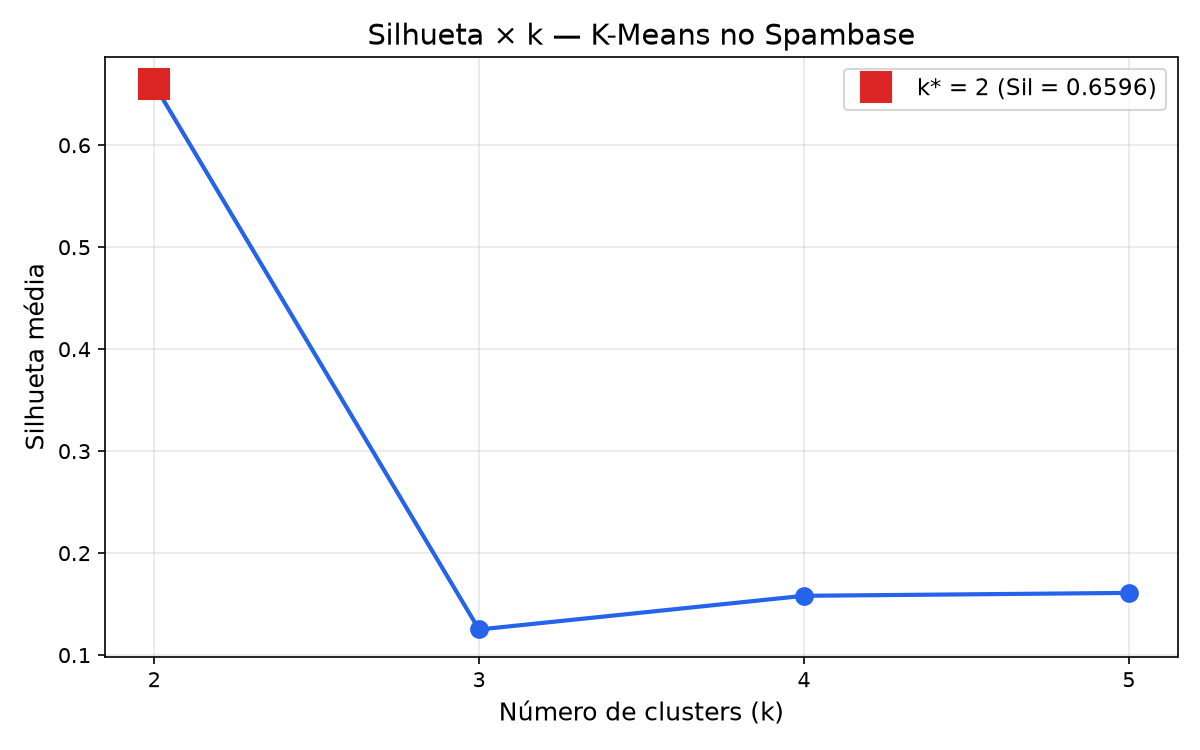
\includegraphics[width=0.7\textwidth]{results/01_silhueta_vs_k.png}
\caption{Silhueta em função de $k$. O ponto em destaque indica $k^{*}=2$.}
\label{fig:silhueta}
\end{figure}

A inércia decresce de forma monotônica com $k$, o que é esperado, já que mais clusters sempre reduzem a distância intra-cluster, e por isso não serve como critério de escolha. A silhueta, por outro lado, é claramente maximizada em $k^{*}=2$ (0.6596), bem acima dos demais valores, o que sugere que a base é mais naturalmente descrita por dois grandes grupos do que por partições mais finas. Um efeito colateral dessa escolha é que os clusters resultantes ficam fortemente desbalanceados: 4567 e-mails (99.3\%) caem no cluster 1 e apenas 34 (0.7\%) no cluster 2. Esse desbalanceamento é o motivo pelo qual optamos pelo F1 ponderado, e não pela acurácia, como critério para a busca de hiperparâmetros e para a comparação entre classificadores.

\subsection{Comparação entre os classificadores}

Com $k^{*}=2$, a tarefa passa a ser uma classificação binária sobre 3680 exemplos de treino e 921 de teste, mantendo em ambos a mesma proporção de 99.3\%/0.7\% entre clusters. A Tabela~\ref{tab:grids} mostra o espaço de hiperparâmetros explorado para cada classificador; a Tabela~\ref{tab:best-params}, a combinação vencedora de cada busca, junto com o F1 médio obtido na validação cruzada (calculado inteiramente sobre o treino, sem qualquer contato com o teste).

\begin{table}[H]
\centering
\small
\caption{Espaço de hiperparâmetros avaliado por classificador (validação cruzada estratificada de 5 folds, otimizando F1 ponderado).}
\label{tab:grids}
\begin{tabular}{@{}l p{8.8cm} r@{}}
\toprule
Classificador & Hiperparâmetros testados & Combinações \\
\midrule
Árvore de Decisão &
\texttt{max\_depth}: \{3, 5, 10, 20, None\}; \texttt{min\_samples\_split}: \{2, 5, 10, 20\}; \texttt{min\_samples\_leaf}: \{1, 2, 5, 10\}; \texttt{criterion}: \{gini, entropy\} & 160 \\[4pt]
Naive Bayes &
\texttt{var\_smoothing}: 7 valores em escala logarítmica entre $10^{-12}$ e $10^{-6}$ & 7 \\[4pt]
Regressão Logística &
\texttt{C}: \{0.01, 0.1, 1, 10, 100\}; \texttt{penalty}: \{l1, l2\}; \texttt{solver}: \{liblinear, saga\}; \texttt{class\_weight}: \{None, balanced\} & 40 \\[4pt]
KNN &
\texttt{n\_neighbors}: \{1, 3, 5, 7, 9, 11, 15, 21\}; \texttt{metric}: \{euclidean, manhattan, chebyshev\}; \texttt{weights}: \{uniform, distance\} & 48 \\[4pt]
Random Forest &
\texttt{n\_estimators}: \{50, 100, 200\}; \texttt{max\_depth}: \{5, 10, 20, None\}; \texttt{min\_samples\_split}: \{2, 5, 10\}; \texttt{min\_samples\_leaf}: \{1, 2, 5\}; \texttt{class\_weight}: \{None, balanced\} & 216 \\
\bottomrule
\end{tabular}
\end{table}

\begin{table}[H]
\centering
\small
\caption{Melhor combinação de hiperparâmetros por classificador e F1 médio na validação cruzada.}
\label{tab:best-params}
\begin{tabular}{@{}l p{8.8cm} r@{}}
\toprule
Classificador & Melhores hiperparâmetros & F1 (CV) \\
\midrule
Árvore de Decisão & \texttt{criterion=entropy, max\_depth=3, min\_samples\_leaf=1, min\_samples\_split=2} & 0.9992 \\
Naive Bayes & \texttt{var\_smoothing=1e-07} & 0.9700 \\
Regressão Logística & \texttt{C=0.1, class\_weight=None, penalty=l2, solver=liblinear} & 0.9997 \\
KNN & \texttt{metric=euclidean, n\_neighbors=15, weights=distance} & 1.0000 \\
Random Forest & \texttt{class\_weight=balanced, max\_depth=5, min\_samples\_leaf=1, min\_samples\_split=2, n\_estimators=50} & 0.9997 \\
\bottomrule
\end{tabular}
\end{table}

Um detalhe interessante é que a busca encontrou modelos bem simples como melhores: a árvore de decisão ideal tem profundidade máxima 3, e a floresta aleatória prefere balancear as classes (\texttt{class\_weight=balanced}) a ficar mais complexa. Isso faz sentido, pois se os clusters já estão bem separados, não é preciso um modelo elaborado para distingui-los.

A Tabela~\ref{tab:test-results} e a Figura~\ref{fig:comparacao} trazem o desempenho de cada classificador no conjunto de teste, isolado durante toda a busca de hiperparâmetros.

\begin{table}[H]
\centering
\caption{Métricas ponderadas no conjunto de teste, por classificador.}
\label{tab:test-results}
\begin{tabular}{@{}l r r r@{}}
\toprule
Classificador & Precision & Recall & F1-score \\
\midrule
Árvore de Decisão & 1.0000 & 1.0000 & 1.0000 \\
Random Forest & 1.0000 & 1.0000 & 1.0000 \\
KNN & 1.0000 & 1.0000 & 1.0000 \\
Regressão Logística & 0.9991 & 0.9989 & 0.9990 \\
Naive Bayes & 0.9919 & 0.9327 & 0.9588 \\
\bottomrule
\end{tabular}
\end{table}

\begin{figure}[H]
\centering
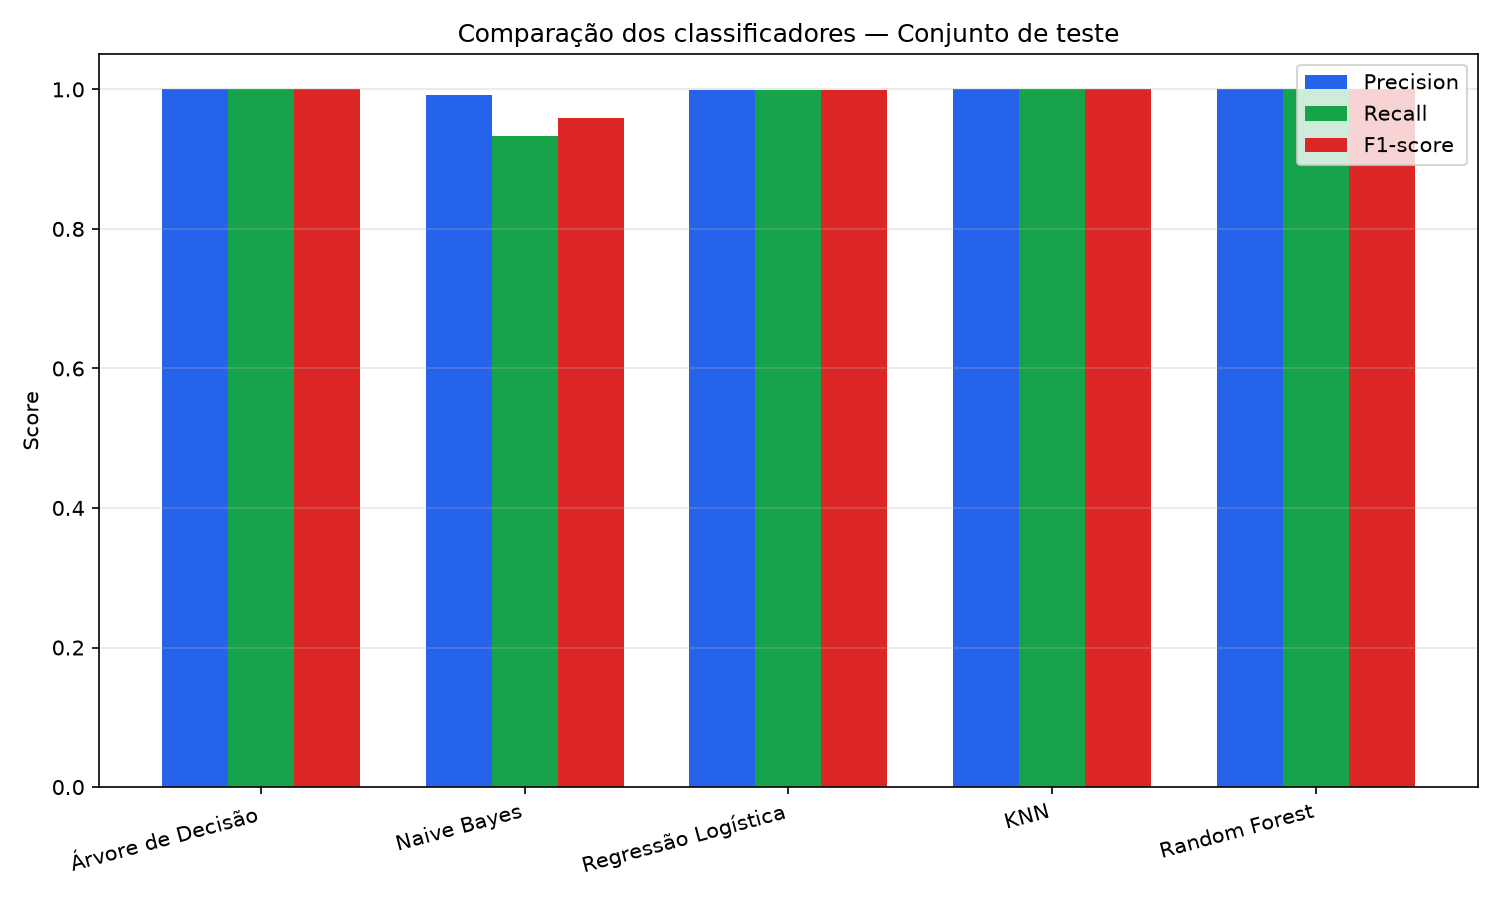
\includegraphics[width=0.85\textwidth]{results/04_comparacao_classificadores.png}
\caption{Comparação de precision, recall e F1-score no conjunto de teste para os cinco classificadores.}
\label{fig:comparacao}
\end{figure}

Árvore de Decisão, Random Forest e KNN atingem desempenho perfeito no teste, e a Regressão Logística fica muito próxima disso (F1 = 0.9990). O Naive Bayes se destaca como o único claramente inferior, com recall de apenas 0.9327, porque sua premissa de independência entre atributos é pouco realista para 57 features de frequência de palavras, que tendem a ser correlacionadas entre si (e-mails com muitas palavras de spam costumam repetir várias delas simultaneamente).

\subsection{Curvas de aprendizagem}

As Figuras~\ref{fig:curva-precision}, \ref{fig:curva-recall} e \ref{fig:curva-f1} mostram como precision, recall e F1-score evoluem no treino (linha tracejada) e no teste (linha sólida) conforme a fração de dados usada para treinar cada classificador aumenta de 5\% para 95\%.

\begin{figure}[H]
\centering
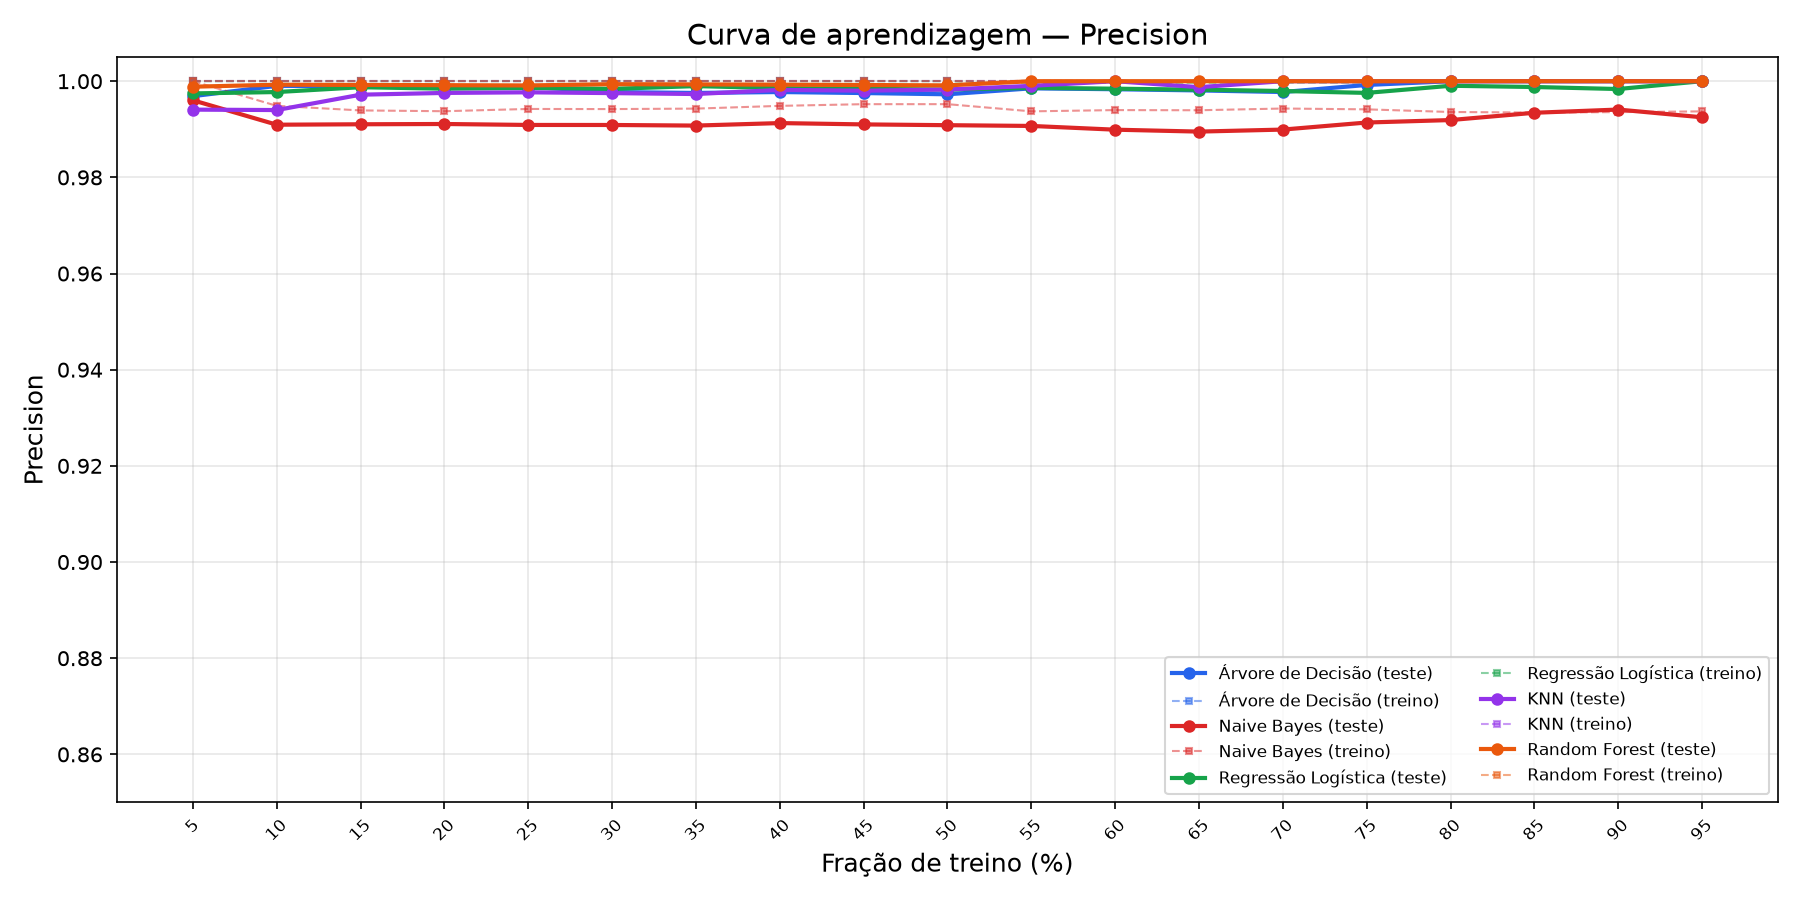
\includegraphics[width=0.85\textwidth]{results/06_curva_aprendizagem_precision.png}
\caption{Curva de aprendizagem para a métrica Precision.}
\label{fig:curva-precision}
\end{figure}

\begin{figure}[H]
\centering
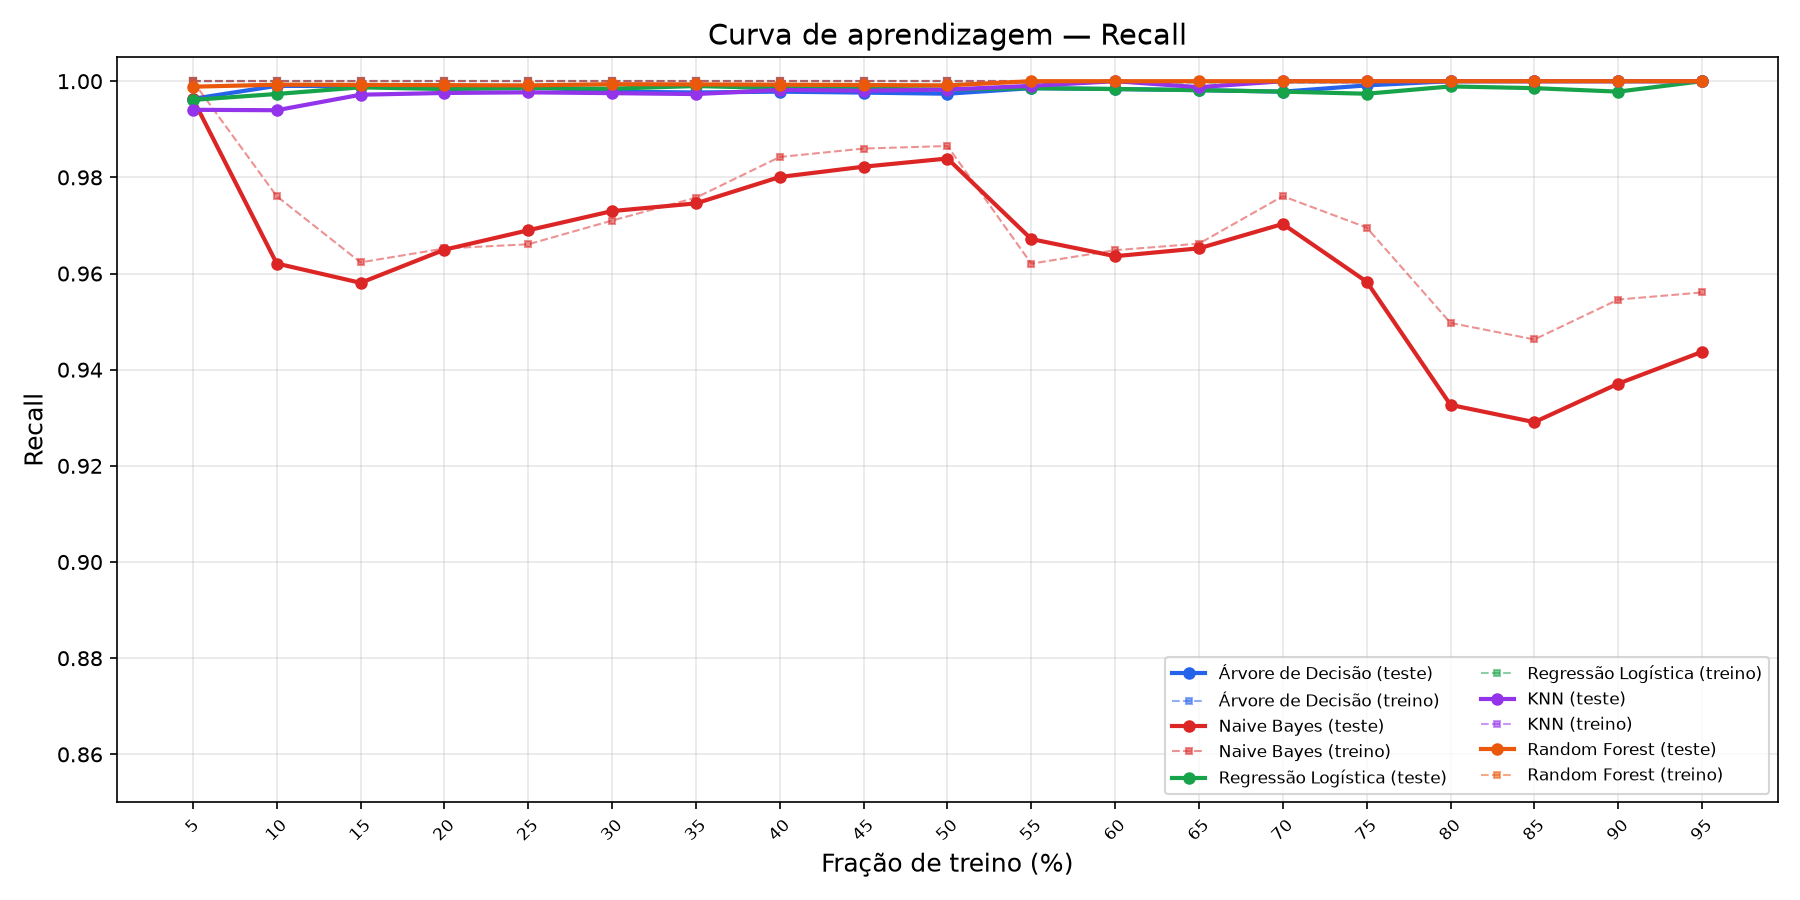
\includegraphics[width=0.85\textwidth]{results/07_curva_aprendizagem_recall.png}
\caption{Curva de aprendizagem para a métrica Recall.}
\label{fig:curva-recall}
\end{figure}

\begin{figure}[H]
\centering
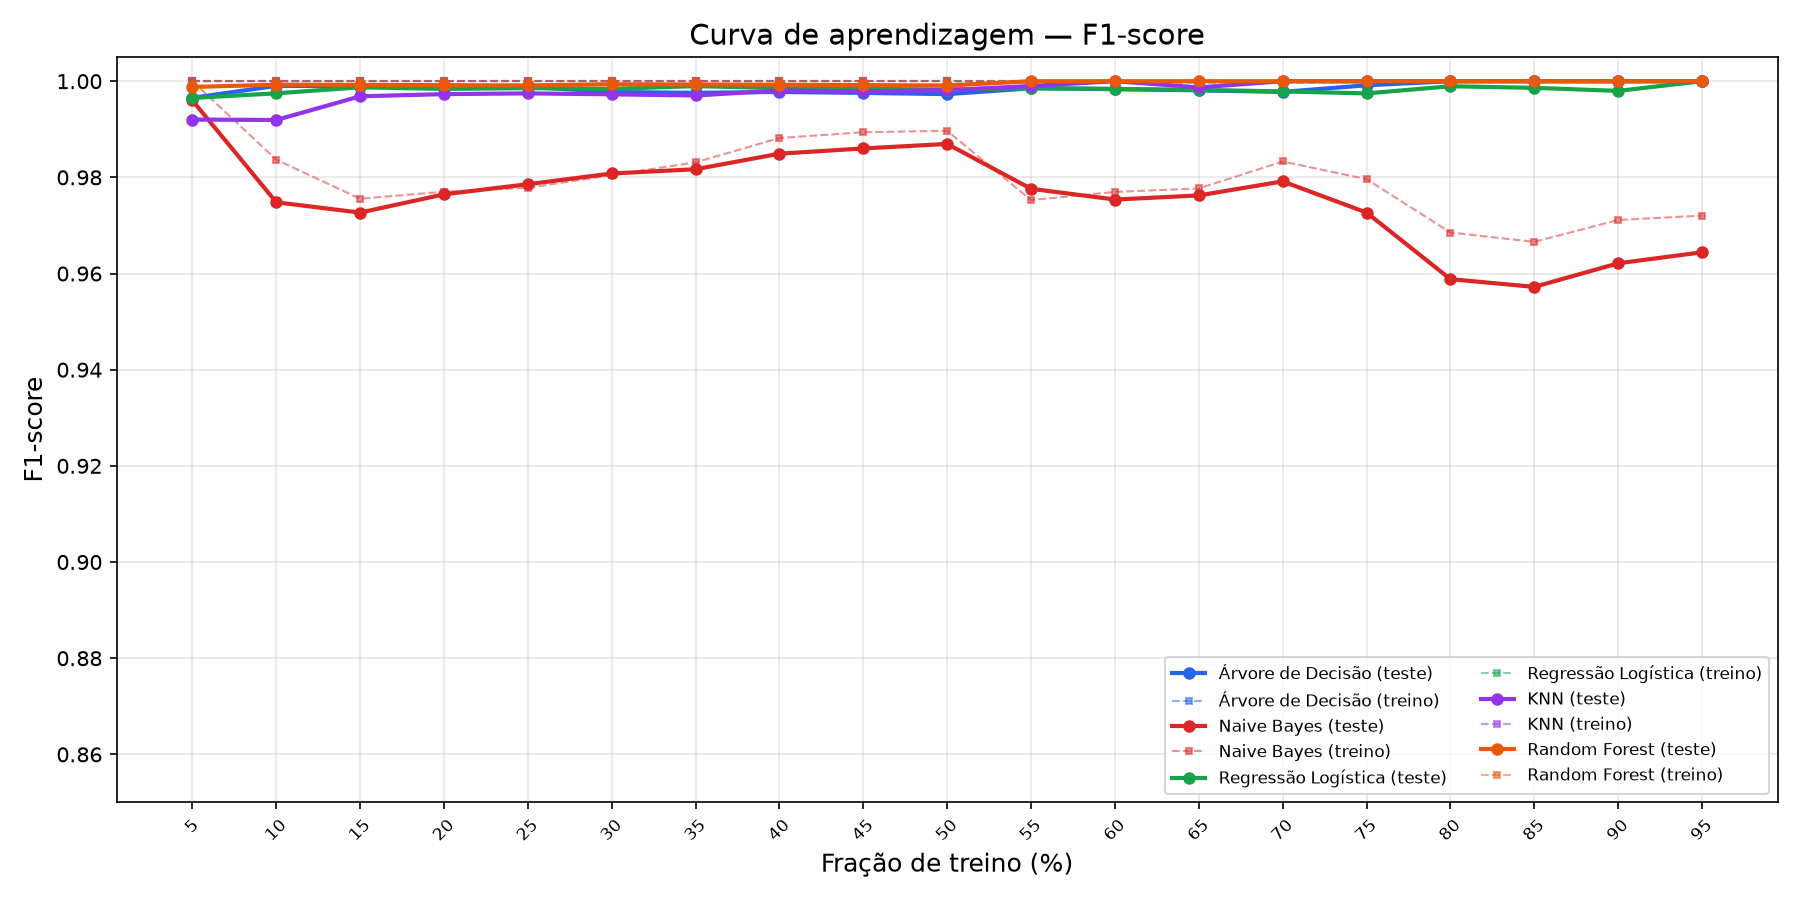
\includegraphics[width=0.85\textwidth]{results/08_curva_aprendizagem_f1score.png}
\caption{Curva de aprendizagem para a métrica F1-score.}
\label{fig:curva-f1}
\end{figure}

O padrão mais evidente é que a maioria dos classificadores atinge desempenho quase perfeito com uma fração pequena de treino, algo em torno de 10\% a 15\% dos dados, porque os clusters usados como classes foram gerados pelo próprio K-Means, algoritmo que por construção maximiza a separação entre grupos, resultando em uma fronteira de decisão simples no espaço normalizado. É por isso também que a silhueta ficou relativamente alta, em 0.66.

Árvore de Decisão, KNN e Random Forest convergem rapidamente para F1 próximo de 1.0, com as curvas de treino e teste praticamente sobrepostas, sem indício de \textit{overfitting}. A Regressão Logística apresenta comportamento semelhante, com F1 de aproximadamente 0.999 no teste. Como a fronteira entre os dois grupos do K-Means é linear, a Regressão Logística tem capacidade de representá-la. Entretanto, seu treinamento não garante encontrar exatamente essa mesma fronteira. A pequena diferença observada pode estar relacionada à amostra de treino e à regularização utilizada, mas o experimento não permite identificar sua causa.

O Naive Bayes é o único caso em que treino e teste não convergem completamente, e seu recall no teste permanece consistentemente mais baixo (em torno de 0.93) mesmo com frações grandes de treino. Isso indica um viés estrutural do modelo, e não falta de dados, já que a suposição de independência entre atributos limita seu desempenho independentemente de quanto treino ele recebe.

Por fim, um ponto interessante é como os modelos lidam com o forte desbalanceamento entre clusters. Com apenas 34 exemplos do cluster minoritário na base inteira, frações de treino de 5\% deixam disponíveis apenas 1 ou 2 exemplos dessa classe, e ainda assim KNN e Random Forest conseguem classificá-los corretamente, o que se explica pelo uso de \texttt{weights=distance} e \texttt{class\_weight=balanced}, respectivamente, ambos pensados justamente para compensar esse tipo de desbalanceamento.

\section{Conclusão}

No fim, o K-Means com $k^{*}=2$ separou a base em dois grupos bem distintos, e essa separação acabou sendo fácil demais para a maioria dos classificadores. Árvore de Decisão, KNN e Random Forest acertaram tudo no teste, a Regressão Logística ficou bem perto disso, e só o Naive Bayes teve um desempenho visivelmente pior, por conta da sua suposição de independência entre atributos, que não se aplica muito bem aqui.

No entanto, vale ressaltar que esse desempenho quase perfeito tem uma explicação simples. Como as próprias classes foram criadas pelo K-Means, um algoritmo que por definição tenta separar os grupos o máximo possível, era esperado que a classificação depois fosse relativamente tranquila. Isso não invalida a comparação entre os classificadores, já que todos enfrentaram o mesmo problema e sob as mesmas condições, mas mostra que esses números não devem ser interpretados como ``os classificadores resolveriam qualquer problema de spam com essa facilidade''. Com o rótulo original de spam da base, por exemplo, provavelmente os resultados seriam mais próximos do mundo real, com mais diferença entre os modelos.

\end{document}
